\documentclass[conference]{IEEEtran}
\IEEEoverridecommandlockouts
% The preceding line is only needed to identify funding in the first footnote. If that is unneeded, please comment it out.
\usepackage{cite}
\usepackage{amsmath,amssymb,amsfonts}
\usepackage{algorithm}
\usepackage{algpseudocode}
\usepackage{graphicx}
\usepackage{textcomp}
\usepackage{xcolor}
\begin{document}


\title{Dynamic Load Balancing of Plasma and Flow Simulations\\
\thanks{
This research was supported by the U.S. Department of Energy, Office of
Science, Office of Advanced Scientific Computing Research, under award
DE-AC52-07NA27344 (FASTMath SciDAC Institute) and by the National Science
Foundation under Grant No.  ACI 1533581, (SI2-SSE: Fast Dynamic Load
Balancing Tools for Extreme Scale Systems).
Any opinions, findings, and conclusions or recommendations expressed in this
material are those of the author(s) and do not necessarily reflect the views
of the National Science Foundation.
}}

\author{\IEEEauthorblockN{1\textsuperscript{st} Gerrett Diamond}
\IEEEauthorblockA{\textit{SCOREC} \\
\textit{Rensselaer Polytechnic Institute}\\
Troy, NY\\
diamog@rpi.edu}
\and
\IEEEauthorblockN{2\textsuperscript{nd} Cameron W. Smith}
\IEEEauthorblockA{\textit{SCOREC} \\
\textit{Rensselaer Polytechnic Institute}\\
Troy, NY\\
smithc11@rpi.edu}
\and
\IEEEauthorblockN{3\textsuperscript{rd} Mark S. Shephard}
\IEEEauthorblockA{\textit{SCOREC} \\
\textit{Rensselaer Polytechnic Institute}\\
Troy, NY\\
shephard@rpi.edu}
}

\maketitle

\begin{abstract}
  Extracting performance from simulations with complex information dependencies
  on massively parallel computers requires the computational work to be evenly
  distributed across the processing resources while maintaining low
  communication costs.
  Plasma simulations using a particle-in-cell method and computational fluid
  dynamics using unstructured mesh-based finite element and volume
  methods present three distinct distribution requirements.
  To meet these needs, we present EnGPar's diffusive partition improvement
  method.
  An initial demonstration of EnGPar's particle distribution improvement is
  provided along with fluid dynamics mesh partition improvement results on up to
  512Ki processes on an IBM BlueGene/Q.
\end{abstract}

\begin{IEEEkeywords}
partition improvement,multigraph,hypergraph,dynamic load balancing,
particle-in-cell, computational fluid dynamics
\end{IEEEkeywords}

\section{Introduction}

High performance computing applications have a wide range of partitioning requirements when
it comes to managing computation and communication costs. For evolving simulations these
costs change as the simulation proceeds. In order to maintain good performance throughout the
simulation, quick repartitioning methods are required that can deal with incremental changes
to the computational load.

In particle in cell (PIC) and computational fluid dynamics (CFD), unstructured meshes are utilized
as a discretization of the spacial domain of interest. The partitioning of mesh results in
computational costs associated with the distribution of the mesh entities and communication
costs relative to the surface area between parts. Special properties for each application
result in further criteria that is critical for performance.

Common partitioning techniques include multilevel graph/hypergraph methods
and geometric methods have been applied to unstructured mesh applications. Multilevel
graph/hypergraph methods are the most powerful tools to build good static partitions
\cite{catalyurek2013umpa,karypis1999parallel,lasalle2013multi,schloegel2002parallel}.
These methods construct a graph representing the data of the application. Then, target
reducing the imbalance (measured as max divided by average) of the graph vertices while
minimizing the edges cut between processes. Multilevel methods are very good at reducing
these metrics, but have a heavy memory cost and can take a long time when scaling out to large
part counts. One way to alleviate these costs is to run multilevel partitioners globally
out to thousands of processes, then partition locally on each of those parts to go out
further. This approach can reach arbitrarily high process counts, but each
local partitioning cannot improve the global partitioning. For meshes, these methods
are good at reducing the imbalance for one mesh entity,
but other mesh entities become greatly imbalanced as the part counts get larger.

Geometric methods are quick spacial methods of partitioning. They are good for getting low
imbalances of a single criteria, but often result in poor surface areas of parts and thus large
communication costs in the applications.

In order to improve the partitions for PIC and CFD applications, we utilize diffusive
load balancing procedures to improve the partitions. Diffusive methods iteratively transfer
weight from heavily loaded parts to lighter neighboring parts
\cite{cybenko1989dynamic,subramanian1994analysis}. Diffusive methods have been shown to be
able to reduce the large imbalances of secondary mesh entities coming out of multilevel
tools \cite{SmithParma2015}. Our tool, EnGPar, uses diffusive methods on a
generalized graph structure in order to improve partitions for a diverse set of application needs.

Section 2 briefly discusses EnGPar. Section 3 discusses a PIC application and initial results
using EnGPar. Section 4 looks at two different types of CFD codes. Results for the CFD
designs is given in section 5. Conclusions and future work are discussed in section 6.

\section{EnGPar}

%\begin{itemize}
%\item Discuss the Ngraph in general graph terms with some figures
%\item Discuss the construction for a element-partitioned mesh as an example with figure
%\item Discuss dynamic load balancing and the general diffusive steps
%\end{itemize}

EnGPar~\cite{engparSC17,engpar_github} is a tool for partition improvement and
dynamic load balancing.
EnGPar utilizes a multi-hypergraph, called the N-graph, to represent the data of
an application in a relational format that allows load balancing of the vertices
and edges simultaneously.
The N-graph is defined as $G^n = \{V, H^n, P^n\}$ where
$V$ is the set of vertices in the graph. The vertices are uniquely assigned to a single
process and are used to represent the main source of data in an application.
$H^n = \{H_1, ..., H_n\}$ are sets of hyperedges where each hyperedge connects a
subset of vertices in $V$. The pins, $P^n = \{P_1,...,P_n\}$, represent the connections from
vertices to hyperedges. Each application that utilizes EnGPar represents the data
that needs partitioning as an N-graph before running any of the partitioning tools.
The general design of the N-graph allows easy representation for different applications
that use structures such as meshes, graphs, and other relational structures.

EnGPar's partition improvement is driven by local diffusive techniques that migrate weight
from heavily weighted parts to lightly weighted parts. This is done by iteratively running
a set of steps until the target imbalance is met or no further improvements can be met.
A diffusive iteration consists of three steps: targeting, selection, and migration.
The targeting step consists of gathering information about the current partition and deciding
which neighbors should be sent weight and how much weight to send. The selection step constructs
a plan of what vertices should be sent to each neighbor in order to satisfy the weights in
the targeting step. The final step, migration, is where the vertices are sent to their
destinations and the partition is changed.

\section{Plasma Simulation}

Plasma physics simulated using a particle-in-cell (PIC) method utilize particles
in the spacial domain of a mesh.
In this work we focus on load balancing the computationally dominant particle
push operation that is common to both passive (e.g., GITR~\cite{younkin2017})
and active (e.g., XGC~\cite{chang2004numerical,Ku2016467,ku2009},
M3D-C1~\cite{jardin2012multiple}, HPIC~\cite{hpic2017}) PIC codes.
Given an initial ABC field on the mesh, the value of the field for each particle
is determined via interpolation from mesh vertices within the maximum
gyro-ring radius of the particle.
The spatial position of the particles is then updated using a push operation.
Particle properties are then interpolated back to the mesh vertices; the reverse
of the vertex-to-particle interpolation process.
Unless the entire mesh is replicated on all processes, particles that do not
have their field dependencies satisfied will need to be
sent to a different process that has sufficient field information.
As these simulations continue the particles become imbalanced and will degrade
performance~\cite{carmona1997,plimptonPic2003,worleyBalancePic2016}.

XGC is a gyrokinetic PIC code for plasma turbulence simulation in a tokamak
fusion device tokamak~\cite{chang2004numerical,Ku2016467,ku2009}.
In this work we refer to a development version of XGC named XGCm that supports
a modified mesh and particle distribution strategy.
XGCm decomposes the domain with a 2D mesh of the
of the polodial plane that is repeated along the toroidal direction.
Figure~\ref{fig:xgcmPtn}-a depicts a simplified representation of the tokamak computational
domain, the polodial planes that decompose it in the toroidal direction, and the
definition of physics-based geometric features within the planes.
Specifically, Figures~\ref{fig:xgcmPtn}-b and ~\ref{fig:xgcmPtn}-c depict the
flux curve and the faces they form.
Figures~\ref{fig:xgcmPtn}-d and ~\ref{fig:xgcmPtn}-e depicts a core and buffer
flux faces, and their assignment to a group.
To satisfy information dependencies of particles belonging to the core,
the sets of elements of neighboring cores are replicated to satisfy
particle data dependencies and thus avoid communication during the
computationally intensive particle push operation.
These replicated elements are referred to as the buffer flux faces.
Note, each process has a copy of the entire group.
This decomposition of the polodial plane is identical for all planes along the
toroidal direction and does does not change during the simulation.

\begin{figure}[!ht]
  \centering
  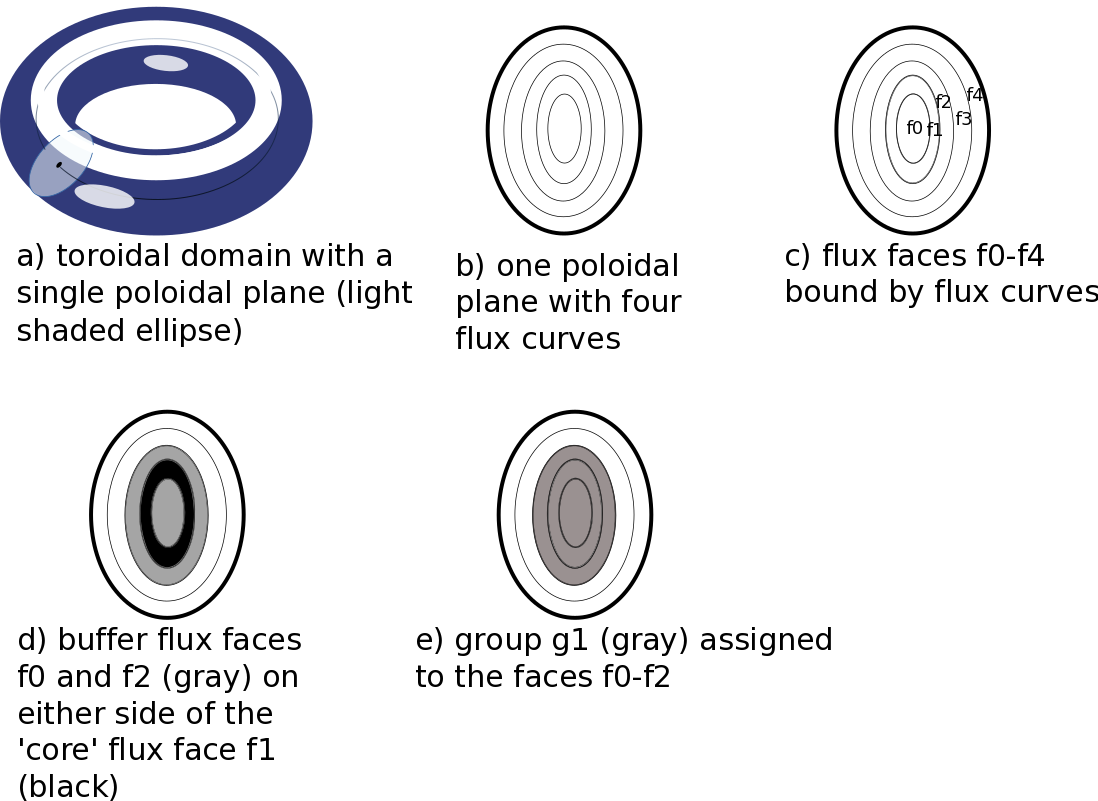
\includegraphics[width=.4\textwidth]{../figures/xgcm_partition.png}
  \caption{XGCm mesh distribution in the toroidal and polodial directions of a tokamak.}
  \label{fig:xgcmPtn}
\end{figure}

The elements in the core assigned to each group, and some layers of the
replicated elements that surround it, are marked as a safe region since there is
sufficient mesh field information available to satisfy the dependency of the
push operation {\color{red} What is the dependency during push on the mesh?}.
Initially, particles are distributed uniformly over each flux face.
The dominant motion of the particles, projected to the polodial plane, tends to
keep them within their initial flux face while a secondary motion drifts them
outwards towards the boundary of the plane.
If the particle moves outside of the safe region it is migrated to a process
where it resides in the safe region.

To ensure that particles are always migrated to the safe elements
of a process, we construct the N-graph carefully such that any partition
decision in EnGPar will always maintain this requirement in XGCM. Towards this,
we represent each region
of overlapping safe zones. Figure \ref{fig:sbars} depicts a model a) with four flux faces labeled
in b) as f0-f3. Safe zones for each \texttt{core} is shown in the second row.
Each overlapping safe zone set, $\bar{S_i}$, is in the third row. For a mesh face in
one of the $\bar{S_i}$, the safe zones in the set represent each group a particle in that element
can migrate to.

The N-graph is then constructed using the set of $\bar{S_i}$. For each $\bar{S_i}$ a
component is constructed consisting of a hyperedge and vertices for each safe zone
$S_j \in \bar{S_i}$. The hyperedge connects each of the vertices in the component.
The fourth row of Figure \ref{fig:sbars} shows the N-graph components for the example model.
Weights are then applied to each vertex based on the number of particles in the elements
for each part. Arbitrary particle counts are labeled within each graph vertex in the figure.
EnGPar is then used in order to determine how to redistribute the particles or weight
on this graph.

\begin{figure}[!ht]
  \centering
  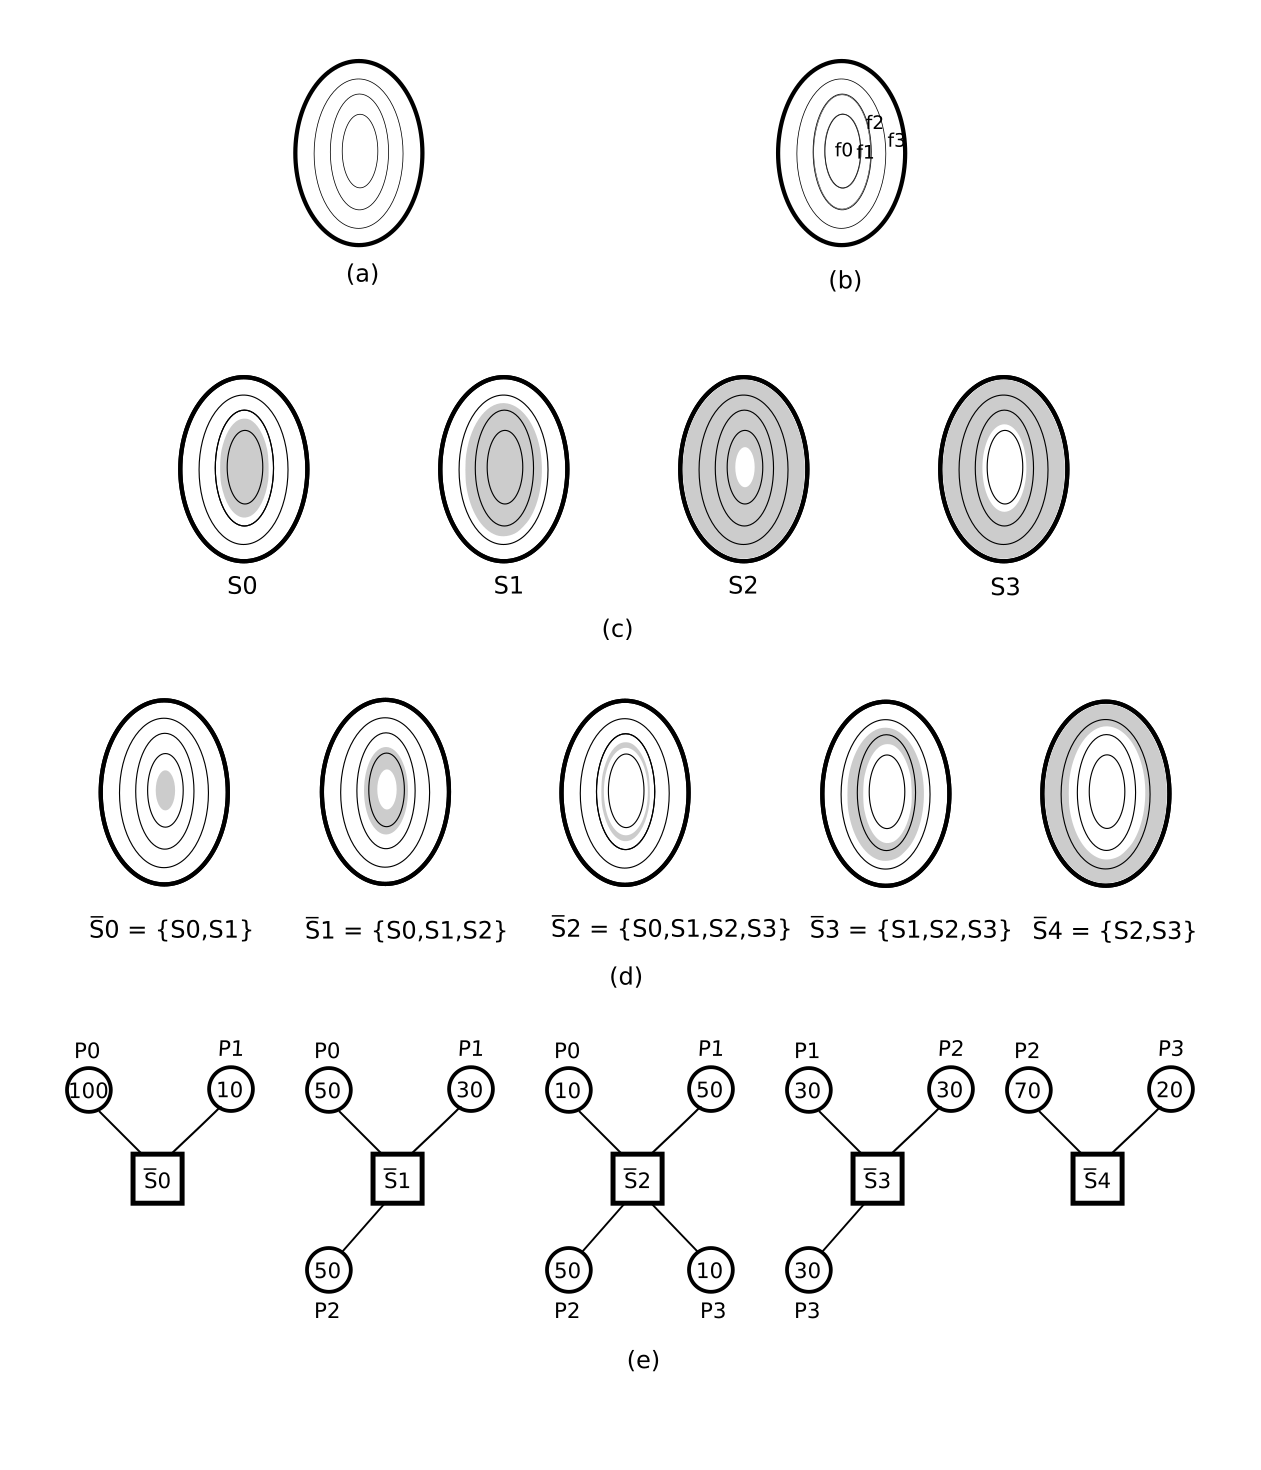
\includegraphics[width=.4\textwidth]{../figures/xgcm_ngraph_construction.png}
  \caption{An example of overlapping safe zones and the N-graph constructed from
  them.{\color{red} Move embedded captions to here}}
  \label{fig:sbars}
\end{figure}

In order to balance the particles in the mesh, we target redistributing the weights within
each component. We run diffusive techniques on the weights of the vertices
rather than the vertices. This means that instead of migrating graph vertices, we migrate the
weight of the vertices across hyperedges to neighboring vertices to reduce the imbalance
of load in the graph.

After EnGPar's weight diffusion is run, a migration plan is returned that details how
much weight to send from each graph vertex on a part to each of its neighboring vertices.
In XGCm, particles are migrated in order to match the plan. Since each graph vertex was only
connected to processes that could receive the particles from the part, any decision XGCm makes
within the $\bar{S_i}$ will satisfy the requirement of particles being in safe zones. Future work
will go into different particle selection methods that can be applied to reduce how often
dynamic load balancing will be required as particles continue to propagate.

Initial demonstrations of the weighted partitioning approach are run on a 16
process test case. The mesh has around four thousand
mesh faces, four flux faces with four processes per flux face and sixteen thousand particles.
The initial partitioning of particles has an imbalance of 42\%. After running EnGPar, the
imbalance of particles is reduced to 18\%. {\color{red} Should the run time be
improved proportionally to the imbalance reduction?}

\section{Computational Fluid Dynamics}

Parallel computational fluid dynamic (CFD) applications using
finite volume and finite elements partition meshes in different
ways to efficiently resolve data dependencies.
A partition of mesh elements uniquely assigns each mesh element to a process.
Lower dimension entities are duplicated as needed to form the closure of the
elements.
For example, if two triangles share an edge, but are assigned to different
processes, the shared edge and its bounding vertices will exist on both
processes.
A vertex-partitioned mesh means that
instead of elements being uniquely assigned to parts, the vertices are, and the elements are
copied along the boundary to any process that shares them. We examine both methods of
partitioning meshes with EnGPar.

\subsection{Element-partitioned mesh}

For element-partitioned meshes, the N-graph is constructed by first representing the mesh elements
as graph vertices. Then, graph hyperedges are constructed for each mesh vertex. Pins
are then created between each hyperedge and graph vertex where the mesh vertex bounds the
mesh element. For higher order finite element simulations, where degrees of freedom are
associated with mesh edges and mesh faces, additional graph hyperedge types can be constructed
similarly for those mesh dimensions. Figure \ref{fig:mesh2graph} shows how a 2-D mesh (a)
is converted into the N-graph with hyperedges as mesh vertices (b) and with hyperedges for
both mesh vertices and mesh edges (c).

\begin{figure}[!ht]
  \centering
  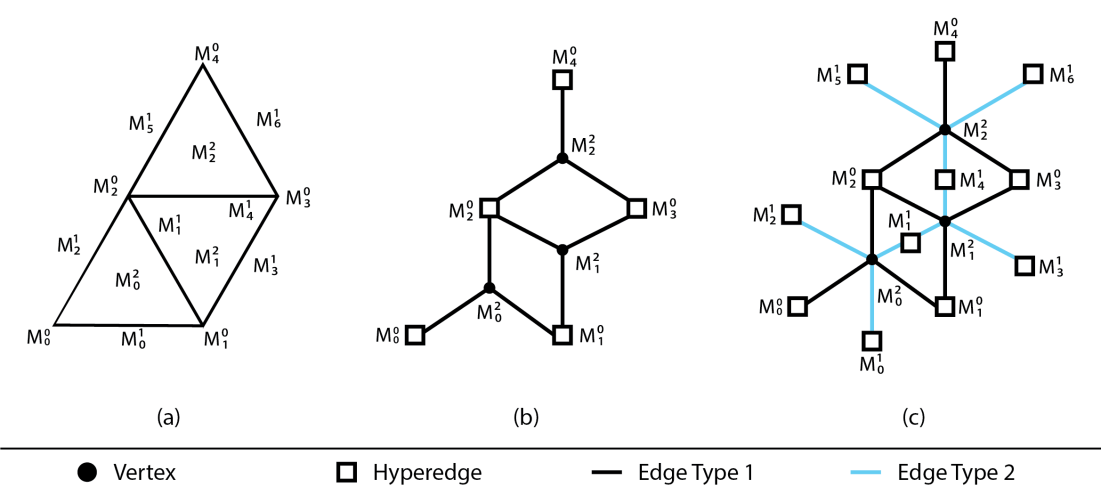
\includegraphics[width=3.5in]{../figures/exampleMesh2Graph.png}
  \caption{(a) a 2D unstructured mesh. (b) N-graph construction with elements$\rightarrow$vertices, vertices$\rightarrow$hyperedges. (c) Same construction, but with an additional edge type for mesh edges.}
  \label{fig:mesh2graph}
\end{figure}

In previous work on this case, we used EnGPar to improve partitions of an
element-partitioned mesh targeting balancing mesh vertices and mesh elements \cite{engparSC17}.
For larger process counts, EnGPar fell short balancing mesh vertices.
We identified that EnGPar was reaching a local minimum due to poor choices of destination part
when selecting graph vertices that were on the part boundary of several processes. In order
to make better decisions, we choose the destination part based on the largest surface area
between the source part and the potential destination part. This results in migrating these
vertices to parts that are more connected to the source part instead of parts that may only
share a few edges.

\subsection{Vertex-partitioned meshes}

To represent the vertex-partitioned mesh in EnGPar, the construction
is essentially the opposite of the element-partitioned mesh. Graph
vertices are defined by mesh vertices and graph hyperedges are defined
by mesh elements. The pins between graph vertices and hyperedges are
created for any mesh vertex that bounds a mesh element.

{\color{red} Add a figure of vertex-partitioned mesh to Ngraph?}

During initial attempts at improving the partitions, we found that the edge cut was growing
at a large rate as we improved edge imbalance. This has been attributed to the differences
caused by the vertex-partitioning of the mesh. For element-partitioned meshes, the hyperedges
represent the mesh vertices. To maintain a low edge cut, mesh vertices that bound many mesh
elements should not be cut across partitions. Towards this, EnGPar avoids migrating cavities
around these high-degree hyperedges. For vertex-partitioned meshes, this problem is reversed
since mesh vertices are represented as graph vertices and hyperedges all have roughly uniform
low degrees based on the element: four in a tetrahedron, five in a pyramid, six in a prism, etc.
Thus the problem of edge cut arises for having high degree graph vertices along the partition
boundary which leads to a larger edge cut.

To control the edge cut while balancing the graph, we introduce a metric to represent the
potential edge cut change for a cavity. The metric is the ratio of hyperedges that will be cut
after the cavity is migrated to the hyperedges currently cut around the cavity. We introduce a
parameter to EnGPar that will only migrate a cavity if the metric is below the given tolerance.
Setting this parameter to 1.0 forces EnGPar to migrate cavities that will not increase the edge
cut locally. This does not guarantee that the edge cut will decrease as the metric does not take
into account other cavities that are migrated in the iteration. Smaller values of this
parameter will limit the increase in edge cut, but also limit EnGPar's ability to improve the
imbalance and either take more iterations to reach the imbalance tolerance or stagnate at a
higher imbalance.

\subsection{Boundary Layer Stacks}

{\color{red} CWS These paragraphs were alienated by merging the two sections so I moved them here. Feel free to move them elsewhere if you think they fit better elsewhere.}
Structured boundary layer element stacks growing from geometric model faces can
be used to reduce discretization errors and reduce mesh element count (i.e., versus
a full unstructured tetrahedral mesh) when there are strong gradients in
principle fields normal to a geometric model surface {\color{red} REFERENCE}.
Figure XYZ depicts the prismatic boundary layer elements along the surface of an
air foil.
Accounting for this structured portion of the mesh during load balancing can
improve the quality of the partition.

{\color{red} GD (if you have a good one in mind) Show a good boundary layer
stack mesh - yes I'll add that in the next commit along with associated
references}

Assigning a stack of boundary layer vertices or
elements to a single process reduces the cut; i.e., cuts that are both normal to
and in-plane with the boundary layer will have more surface area than a cut that
is only along the planar or normal direction.
However, partitioners
operating on the graph formed by the dual of the mesh, will separate
the boundary stacks. For a vertex partition, we combine the mesh vertices of each stack into one graph vertex
during construction of the N-graph to prevent separation of stacks and the
resulting high surface area cuts. 

Algorithm \ref{alg:collapse} details steps taken to
combine the stacks. The algorithm loops over each vertex classified on a geometric
model face to see if it bounds a prism on lines 1-2. From each of these vertices, the
algorithm iteratively walks up mesh edges that do not bound any triangles on lines 3-14. An edge
that only bounds quad faces is guaranteed to be the edge going up the prism elements. Once
a tetrahedron or pyramid element is hit there will be no edges that are not adjacent to a triangle
and the iteration will end.
\begin{algorithm}
  \caption{Boundary Layer Stack Collapse}
  \label{alg:collapse}
  \small
  \begin{algorithmic}[1]
    \ForAll{Vertices, $v$, classified on a geometric model face}
    \If{$v$ bounds a prism}
    \State $prev\_edge = NULL$
    \State $next\_edge = NULL$
    \ForAll{Edges, $e$, bounded by $v$}
    \If{$e$ bounds no triangles and is not $prev\_edge$}
    \State $next\_edge = e$
    \EndIf
    \EndFor
    \If{$next\_edge$ is not $NULL$}
    \State $edge\_prev = e$
    \State $v = other\_vertex(v,e$)
    \State goto 4:
    \EndIf
    \EndIf
    \EndFor
  \end{algorithmic}
\end{algorithm}

To maintain the correct computational and communication load of the stacks,
we assign weights to the vertices and hyperedges that result from the stack. Each boundary layer
stack vertex is given a weight equal to the number of vertices in the stack, and the hyperedges
are given a weight of the number of elements that share the same graph vertices. All other
graph vertices and hyperedges are given a weight of one.


\section{Results}
\begin{itemize}
\item PIC
\begin{itemize}
  \item engpar vs no balancing timing and particle imbalance
\end{itemize}
\item FUN3D
\begin{itemize}
  \item aepw with and without BL collapse
  \item engpar parmetis (no BL collapse) vs fun3d parmetis(?) - need fun3d 
    solver counts of vertices and edges to compute its imbalance - done
  \item engpar parmetis (no BL collapse) + vtx improvement vs engpar parmetis
  \item engpar parmetis (no BL collapse) + vtx > elm improvement vs engpar parmetis
\end{itemize}
\end{itemize}

\subsection{Element-partitioned mesh}

Tests for the finite element case were run with a one billion element mesh of an airplane's
vertical tail structure. EnGPar was run on the Mira BlueGene/Q system at the Argonne Leadership
Computing Facility \cite{haring2012ibm} on partitions from 128Ki ($128*2^{10}$) up to 512Ki parts.
These partitions were created by using ParMETIS part k-way \cite{karypis1999parallel} globally
up to 8Ki parts. Then METIS is run on each part locally to create the final partitions.
The initial mesh element imbalance is 2\% and the mesh vertex imbalance ranges from 12\% for
the 128Ki partition up to 53\% at 512Ki parts.

We compare EnGPar to ParMA \cite{SmithParma2015}, a diffusive load balancer that
works directly on an unstructured mesh.
Each tool is run on the partitions to balance the mesh vertices down to 5\% while keeping the mesh
element imbalance below 5\%. Figures \ref{fig:fem_vtximb} shows the mesh vertex imbalance after
ParMETIS and after EnGPar and ParMA are used. Both tools significantly reduce the mesh vertex
imbalance. For the 128Ki and 256Ki cases, both reduce the imbalance to the target 5\%. In
the 512Ki case, EnGPar reduces the mesh vertex imbalance to 6\% while ParMA reduces to the
target.

{\color{red} If we keep the discussion of previous results we should add the old EnGPar results in the plot? CWS do you think it is worth including the old results for further comparison?}
\begin{figure}[!ht]
  \centering
  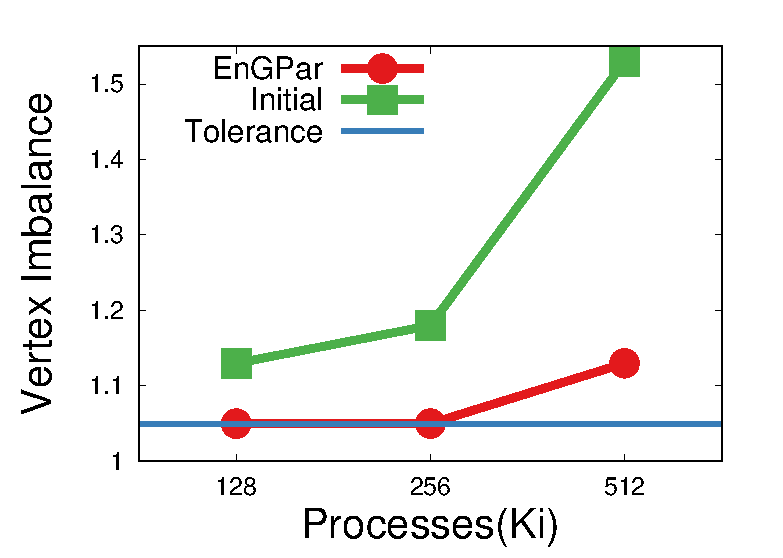
\includegraphics[width=3in]{plots/mira_fem_results/vimb_v_cores}
  \caption{Vertex imbalance for the initial partitioning and the partitions created by
    EnGPar and ParMA. Element imbalance is maintained below the 5\% tolerance for all cases.}
  \label{fig:fem_vtximb}
\end{figure}

Figure \ref{fig:fem_time} shows the runtime for each partition of ParMA and EnGPar. The
timing for EnGPar includes the construction of the N-graph and subsequent repartition of
the mesh after running EnGPar to fairly compare with ParMA which doesn't require any
conversions of the mesh. In all cases EnGPar runs faster. The speedup ranges from
25\% faster at the 256Ki case up to 54\% faster for the 512Ki partition.

\begin{figure}[!ht]
  \centering
  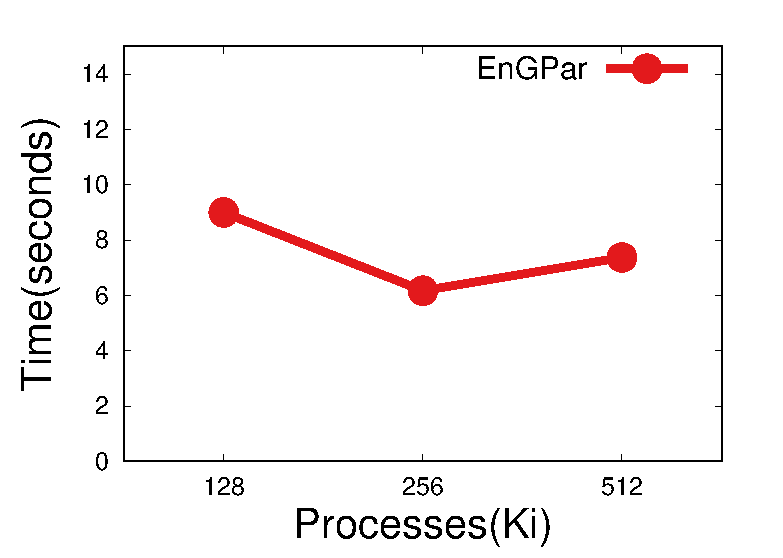
\includegraphics[width=3in]{plots/mira_fem_results/time_v_cores}
  \caption{Time to balance for EnGPar and ParMA}
  \label{fig:fem_time}
\end{figure}

\subsection {Vertex-partitioned mesh}
Experiments for the vertex-partitioned mesh application were done with a 60 million
element mesh on 1024 to 8192 processes. To show the affect of the edge cut
metric, we ran the same test for each process count giving values for the metric
from 0.5 to 1.2 as well as the metric being turned off. Each test runs 30 iterations
of EnGPar's edge balancer while strictly maintaining the vertex imbalance at 5\%.
{\color{red} As per our previous discussion about imbalance, the plots are not adjusted yet to
  match this definition of imbalance. Neither are the stat described below.}
In order to better isolate the edge cut from edge imbalance, we measure edge imbalance as the
maximum edges on a process divided by the average edge of the initial partition.
Figure \ref{fig:metric} shows the edge cut and edge imbalances for each
test. The initial stats after ParMETIS has partitioned the mesh are also provided. For the
8192 part case, without
the metric used, EnGPar reduces the edge imbalance by 24\% while increasing the cut by
34\%. Turning on the metric with a value of 1.2 results in limiting the increase of the cut to
17\% while reducing the imbalance by 18\%. Results for the metric limit set to 1.0
and 0.8 have similar results following the trend that lower values of the limit result
in lower edge cuts and higher edge imbalance. When the limit is set to 0.5, the edge cut
increases by only 1\% while reducing the imbalance by 11\%.

\begin{figure}[!ht]
  \centering
  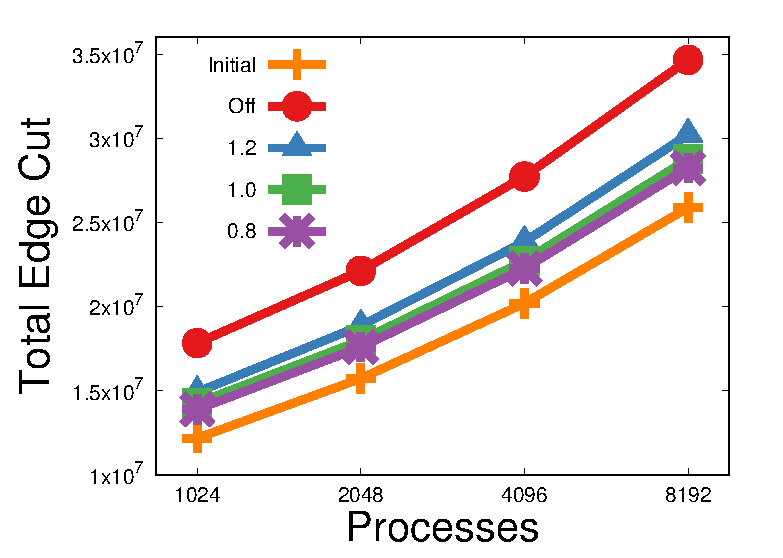
\includegraphics[width=3in]{plots/aepw_edgeCut_collapse_results/ecut_v_cores}
  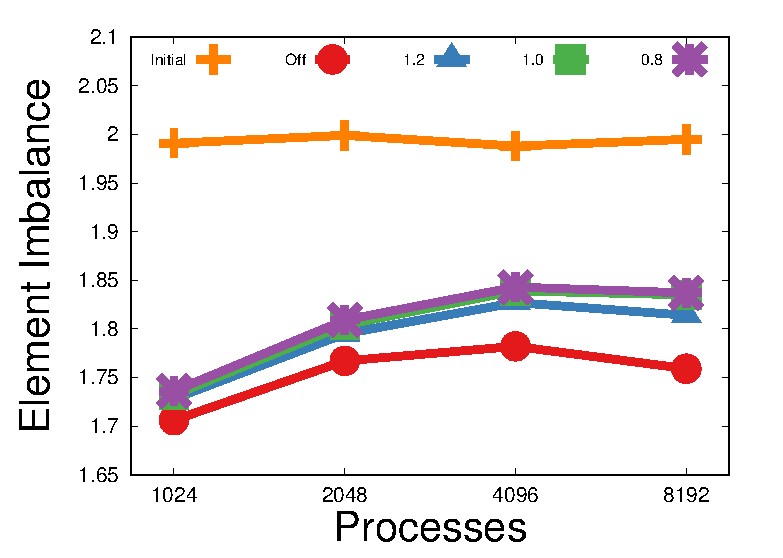
\includegraphics[width=3in]{plots/aepw_edgeCut_collapse_results/eimb_v_cores}
  \caption{Edge cut and imbalance for various values of the metric used to reduce the growth of edge cut. Initial values from ParMETIS and not using the metric are also provided. Vertex imbalance is 5\% for all cases.}
  \label{fig:metric}
\end{figure}

The best configuration from these results is very application specific. The increase in
edge cut means that there will be overall more elements on each part as well as the communication
between parts increases. If communication dominates a simulations scaling then the increase in
edge cut may not be tolerable for the gains on imbalance. So the partition from ParMETIS may
be the best choice or running EnGPar with a low limit for the cut growth metric like in the
0.5 case. However, if the application is very susceptible to imbalance, then a increase in the
edge cut would be worth the decreases in imbalance as seen in the 0.8 - 1.2 cases.

For the boundary layer collapse, we use the same 60 million element mesh. The N-graph is
built in serial from the mesh with the collapsed boundary layers and partitioned
out using global ParMETIS for the 1024 to 8192 partitions.
Then, EnGPar is run for 30 iterations to reduce the edge imbalance. Figure \ref{fig:collapse}
shows the edge cut and edge imbalance after partitioning with
ParMETIS and after EnGPar. {\color{red} Insert discussion about the results.}


\begin{figure}[!ht]
  \centering
  \includegraphics[width=3in]{plots/aepw_edgeCut_collapse_results/ecut_v_cores_collapse}
  \includegraphics[width=3in]{plots/aepw_edgeCut_collapse_results/eimb_v_cores_collapse}
  \caption{Edge cut and imbalance for the graph with collapsed boundary layer stacks. Initial values from ParMETIS are provided. Vertex imbalance is 5\% for all cases.}
  \label{fig:collapse}
\end{figure}

\section{Closing Remarks}
foo

\begin{itemize}
\item accelerators
\item BL collapse
\end{itemize}

\bibliographystyle{IEEEtran}
\bibliography{scorec-refs/scorec-refs}

\end{document}
